\begin{figure}
    \centering

    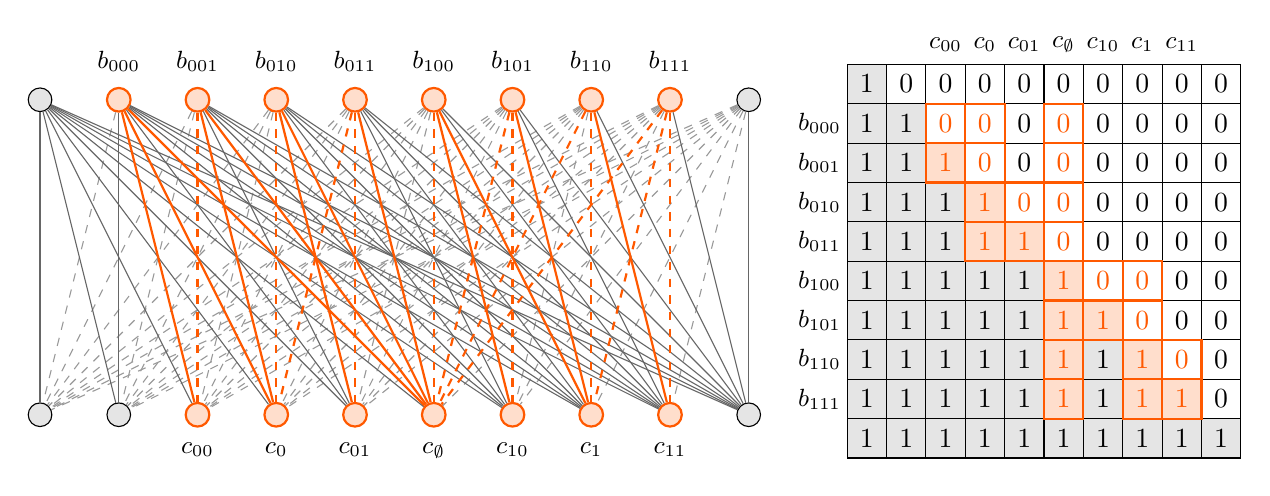
\begin{tikzpicture}[
        vertex/.style={circle, draw, fill=gray!20, minimum size=0.3 cm, inner sep=1pt},
        tree_vertex/.style={circle, thick, draw=orange!70!red, fill=orange!70!red!20, minimum size=0.3 cm, inner sep=1pt},
        label_a/.style={above=2pt, font=\small},
        label_b/.style={below=2pt, font=\small},
        node distance=1.5cm,
        solid edge/.style={draw, thick, black!60},
        dashed edge/.style={draw, dashed, thick, black!40},
        matrix cell/.style={draw, minimum size=0.5 cm, inner sep=0pt},
        matrix label/.style={font=\small, anchor=center}
    ]
	\node[vertex] (a_1) at (1,0) {};
	\node[tree_vertex] (a_2) at (2,0) {};
	\node[tree_vertex] (a_3) at (3,0) {};
	\node[tree_vertex] (a_4) at (4,0) {};
	\node[tree_vertex] (a_5) at (5,0) {};
	\node[tree_vertex] (a_6) at (6,0) {};
	\node[tree_vertex] (a_7) at (7,0) {};
	\node[tree_vertex] (a_8) at (8,0) {};
	\node[tree_vertex] (a_9) at (9,0) {};
	\node[vertex] (a_10) at (10,0) {};
	\node[vertex] (b_1) at (1,-4) {};
	\node[vertex] (b_2) at (2,-4) {};
	\node[tree_vertex] (b_3) at (3,-4) {};
	\node[tree_vertex] (b_4) at (4,-4) {};
	\node[tree_vertex] (b_5) at (5,-4) {};
	\node[tree_vertex] (b_6) at (6,-4) {};
	\node[tree_vertex] (b_7) at (7,-4) {};
	\node[tree_vertex] (b_8) at (8,-4) {};
	\node[tree_vertex] (b_9) at (9,-4) {};
	\node[vertex] (b_10) at (10,-4) {};
	\draw[solid edge, thin] (a_1) -- (b_1);
	\draw[dashed edge, thin] (a_2) -- (b_1);
	\draw[dashed edge, thin] (a_3) -- (b_1);
	\draw[dashed edge, thin] (a_4) -- (b_1);
	\draw[dashed edge, thin] (a_5) -- (b_1);
	\draw[dashed edge, thin] (a_6) -- (b_1);
	\draw[dashed edge, thin] (a_7) -- (b_1);
	\draw[dashed edge, thin] (a_8) -- (b_1);
	\draw[dashed edge, thin] (a_9) -- (b_1);
	\draw[dashed edge, thin] (a_10) -- (b_1);
	\draw[solid edge, thin] (a_1) -- (b_2);
	\draw[solid edge, thin] (a_2) -- (b_2);
	\draw[dashed edge, thin] (a_3) -- (b_2);
	\draw[dashed edge, thin] (a_4) -- (b_2);
	\draw[dashed edge, thin] (a_5) -- (b_2);
	\draw[dashed edge, thin] (a_6) -- (b_2);
	\draw[dashed edge, thin] (a_7) -- (b_2);
	\draw[dashed edge, thin] (a_8) -- (b_2);
	\draw[dashed edge, thin] (a_9) -- (b_2);
	\draw[dashed edge, thin] (a_10) -- (b_2);
	\draw[solid edge, thin] (a_1) -- (b_3);
	\draw[dashed edge, thin] (a_4) -- (b_3);
	\draw[dashed edge, thin] (a_5) -- (b_3);
	\draw[dashed edge, thin] (a_6) -- (b_3);
	\draw[dashed edge, thin] (a_7) -- (b_3);
	\draw[dashed edge, thin] (a_8) -- (b_3);
	\draw[dashed edge, thin] (a_9) -- (b_3);
	\draw[dashed edge, thin] (a_10) -- (b_3);
	\draw[solid edge, thin] (a_1) -- (b_4);
	\draw[dashed edge, thin] (a_6) -- (b_4);
	\draw[dashed edge, thin] (a_7) -- (b_4);
	\draw[dashed edge, thin] (a_8) -- (b_4);
	\draw[dashed edge, thin] (a_9) -- (b_4);
	\draw[dashed edge, thin] (a_10) -- (b_4);
	\draw[solid edge, thin] (a_1) -- (b_5);
	\draw[solid edge, thin] (a_2) -- (b_5);
	\draw[solid edge, thin] (a_3) -- (b_5);
	\draw[dashed edge, thin] (a_6) -- (b_5);
	\draw[dashed edge, thin] (a_7) -- (b_5);
	\draw[dashed edge, thin] (a_8) -- (b_5);
	\draw[dashed edge, thin] (a_9) -- (b_5);
	\draw[dashed edge, thin] (a_10) -- (b_5);
	\draw[solid edge, thin] (a_1) -- (b_6);
	\draw[dashed edge, thin] (a_10) -- (b_6);
	\draw[solid edge, thin] (a_1) -- (b_7);
	\draw[solid edge, thin] (a_2) -- (b_7);
	\draw[solid edge, thin] (a_3) -- (b_7);
	\draw[solid edge, thin] (a_4) -- (b_7);
	\draw[solid edge, thin] (a_5) -- (b_7);
	\draw[dashed edge, thin] (a_8) -- (b_7);
	\draw[dashed edge, thin] (a_9) -- (b_7);
	\draw[dashed edge, thin] (a_10) -- (b_7);
	\draw[solid edge, thin] (a_1) -- (b_8);
	\draw[solid edge, thin] (a_2) -- (b_8);
	\draw[solid edge, thin] (a_3) -- (b_8);
	\draw[solid edge, thin] (a_4) -- (b_8);
	\draw[solid edge, thin] (a_5) -- (b_8);
	\draw[dashed edge, thin] (a_10) -- (b_8);
	\draw[solid edge, thin] (a_1) -- (b_9);
	\draw[solid edge, thin] (a_2) -- (b_9);
	\draw[solid edge, thin] (a_3) -- (b_9);
	\draw[solid edge, thin] (a_4) -- (b_9);
	\draw[solid edge, thin] (a_5) -- (b_9);
	\draw[solid edge, thin] (a_6) -- (b_9);
	\draw[solid edge, thin] (a_7) -- (b_9);
	\draw[dashed edge, thin] (a_10) -- (b_9);
	\draw[solid edge, thin] (a_1) -- (b_10);
	\draw[solid edge, thin] (a_2) -- (b_10);
	\draw[solid edge, thin] (a_3) -- (b_10);
	\draw[solid edge, thin] (a_4) -- (b_10);
	\draw[solid edge, thin] (a_5) -- (b_10);
	\draw[solid edge, thin] (a_6) -- (b_10);
	\draw[solid edge, thin] (a_7) -- (b_10);
	\draw[solid edge, thin] (a_8) -- (b_10);
	\draw[solid edge, thin] (a_9) -- (b_10);
	\draw[solid edge, thin] (a_10) -- (b_10);
	\draw[solid edge, thick, orange!70!red] (a_2) -- (b_3);
	\draw[dashed edge, thick, orange!70!red] (a_3) -- (b_3);
	\draw[solid edge, thick, orange!70!red] (a_2) -- (b_4);
	\draw[solid edge, thick, orange!70!red] (a_3) -- (b_4);
	\draw[dashed edge, thick, orange!70!red] (a_4) -- (b_4);
	\draw[dashed edge, thick, orange!70!red] (a_5) -- (b_4);
	\draw[solid edge, thick, orange!70!red] (a_4) -- (b_5);
	\draw[dashed edge, thick, orange!70!red] (a_5) -- (b_5);
	\draw[solid edge, thick, orange!70!red] (a_2) -- (b_6);
	\draw[solid edge, thick, orange!70!red] (a_3) -- (b_6);
	\draw[solid edge, thick, orange!70!red] (a_4) -- (b_6);
	\draw[solid edge, thick, orange!70!red] (a_5) -- (b_6);
	\draw[dashed edge, thick, orange!70!red] (a_6) -- (b_6);
	\draw[dashed edge, thick, orange!70!red] (a_7) -- (b_6);
	\draw[dashed edge, thick, orange!70!red] (a_8) -- (b_6);
	\draw[dashed edge, thick, orange!70!red] (a_9) -- (b_6);
	\draw[solid edge, thick, orange!70!red] (a_6) -- (b_7);
	\draw[dashed edge, thick, orange!70!red] (a_7) -- (b_7);
	\draw[solid edge, thick, orange!70!red] (a_6) -- (b_8);
	\draw[solid edge, thick, orange!70!red] (a_7) -- (b_8);
	\draw[dashed edge, thick, orange!70!red] (a_8) -- (b_8);
	\draw[dashed edge, thick, orange!70!red] (a_9) -- (b_8);
	\draw[solid edge, thick, orange!70!red] (a_8) -- (b_9);
	\draw[dashed edge, thick, orange!70!red] (a_9) -- (b_9);
	\node[label_a] at (a_2.north) {$b_{000}$};
	\node[label_a] at (a_3.north) {$b_{001}$};
	\node[label_a] at (a_4.north) {$b_{010}$};
	\node[label_a] at (a_5.north) {$b_{011}$};
	\node[label_a] at (a_6.north) {$b_{100}$};
	\node[label_a] at (a_7.north) {$b_{101}$};
	\node[label_a] at (a_8.north) {$b_{110}$};
	\node[label_a] at (a_9.north) {$b_{111}$};
	\node[label_b] at (b_3.south) {$c_{00}$};
	\node[label_b] at (b_4.south) {$c_{0}$};
	\node[label_b] at (b_5.south) {$c_{01}$};
	\node[label_b] at (b_6.south) {$c_{\emptyset}$};
	\node[label_b] at (b_7.south) {$c_{10}$};
	\node[label_b] at (b_8.south) {$c_{1}$};
	\node[label_b] at (b_9.south) {$c_{11}$};

\begin{scope}[xshift=12 cm]
		\node[matrix cell, fill=gray!20] at (-0.5, 0.19999999999999996) {1};
		\node[matrix cell, fill=gray!20] at (-0.5, -0.30000000000000004) {1};
		\node[matrix cell, fill=gray!20] at (-0.5, -0.8) {1};
		\node[matrix cell, fill=gray!20] at (-0.5, -1.3) {1};
		\node[matrix cell, fill=gray!20] at (-0.5, -1.8) {1};
		\node[matrix cell, fill=gray!20] at (-0.5, -2.3) {1};
		\node[matrix cell, fill=gray!20] at (-0.5, -2.8) {1};
		\node[matrix cell, fill=gray!20] at (-0.5, -3.3) {1};
		\node[matrix cell, fill=gray!20] at (-0.5, -3.8) {1};
		\node[matrix cell, fill=gray!20] at (-0.5, -4.3) {1};
		\node[matrix cell] at (0.0, 0.19999999999999996) {0};
		\node[matrix cell, fill=gray!20] at (0.0, -0.30000000000000004) {1};
		\node[matrix cell, fill=gray!20] at (0.0, -0.8) {1};
		\node[matrix cell, fill=gray!20] at (0.0, -1.3) {1};
		\node[matrix cell, fill=gray!20] at (0.0, -1.8) {1};
		\node[matrix cell, fill=gray!20] at (0.0, -2.3) {1};
		\node[matrix cell, fill=gray!20] at (0.0, -2.8) {1};
		\node[matrix cell, fill=gray!20] at (0.0, -3.3) {1};
		\node[matrix cell, fill=gray!20] at (0.0, -3.8) {1};
		\node[matrix cell, fill=gray!20] at (0.0, -4.3) {1};
		\node[matrix cell] at (0.5, 0.19999999999999996) {0};
		\node[matrix cell, fill=gray!20] at (0.5, -1.3) {1};
		\node[matrix cell, fill=gray!20] at (0.5, -1.8) {1};
		\node[matrix cell, fill=gray!20] at (0.5, -2.3) {1};
		\node[matrix cell, fill=gray!20] at (0.5, -2.8) {1};
		\node[matrix cell, fill=gray!20] at (0.5, -3.3) {1};
		\node[matrix cell, fill=gray!20] at (0.5, -3.8) {1};
		\node[matrix cell, fill=gray!20] at (0.5, -4.3) {1};
		\node[matrix cell] at (1.0, 0.19999999999999996) {0};
		\node[matrix cell, fill=gray!20] at (1.0, -2.3) {1};
		\node[matrix cell, fill=gray!20] at (1.0, -2.8) {1};
		\node[matrix cell, fill=gray!20] at (1.0, -3.3) {1};
		\node[matrix cell, fill=gray!20] at (1.0, -3.8) {1};
		\node[matrix cell, fill=gray!20] at (1.0, -4.3) {1};
		\node[matrix cell] at (1.5, 0.19999999999999996) {0};
		\node[matrix cell] at (1.5, -0.30000000000000004) {0};
		\node[matrix cell] at (1.5, -0.8) {0};
		\node[matrix cell, fill=gray!20] at (1.5, -2.3) {1};
		\node[matrix cell, fill=gray!20] at (1.5, -2.8) {1};
		\node[matrix cell, fill=gray!20] at (1.5, -3.3) {1};
		\node[matrix cell, fill=gray!20] at (1.5, -3.8) {1};
		\node[matrix cell, fill=gray!20] at (1.5, -4.3) {1};
		\node[matrix cell] at (2.0, 0.19999999999999996) {0};
		\node[matrix cell, fill=gray!20] at (2.0, -4.3) {1};
		\node[matrix cell] at (2.5, 0.19999999999999996) {0};
		\node[matrix cell] at (2.5, -0.30000000000000004) {0};
		\node[matrix cell] at (2.5, -0.8) {0};
		\node[matrix cell] at (2.5, -1.3) {0};
		\node[matrix cell] at (2.5, -1.8) {0};
		\node[matrix cell, fill=gray!20] at (2.5, -3.3) {1};
		\node[matrix cell, fill=gray!20] at (2.5, -3.8) {1};
		\node[matrix cell, fill=gray!20] at (2.5, -4.3) {1};
		\node[matrix cell] at (3.0, 0.19999999999999996) {0};
		\node[matrix cell] at (3.0, -0.30000000000000004) {0};
		\node[matrix cell] at (3.0, -0.8) {0};
		\node[matrix cell] at (3.0, -1.3) {0};
		\node[matrix cell] at (3.0, -1.8) {0};
		\node[matrix cell, fill=gray!20] at (3.0, -4.3) {1};
		\node[matrix cell] at (3.5, 0.19999999999999996) {0};
		\node[matrix cell] at (3.5, -0.30000000000000004) {0};
		\node[matrix cell] at (3.5, -0.8) {0};
		\node[matrix cell] at (3.5, -1.3) {0};
		\node[matrix cell] at (3.5, -1.8) {0};
		\node[matrix cell] at (3.5, -2.3) {0};
		\node[matrix cell] at (3.5, -2.8) {0};
		\node[matrix cell, fill=gray!20] at (3.5, -4.3) {1};
		\node[matrix cell] at (4.0, 0.19999999999999996) {0};
		\node[matrix cell] at (4.0, -0.30000000000000004) {0};
		\node[matrix cell] at (4.0, -0.8) {0};
		\node[matrix cell] at (4.0, -1.3) {0};
		\node[matrix cell] at (4.0, -1.8) {0};
		\node[matrix cell] at (4.0, -2.3) {0};
		\node[matrix cell] at (4.0, -2.8) {0};
		\node[matrix cell] at (4.0, -3.3) {0};
		\node[matrix cell] at (4.0, -3.8) {0};
		\node[matrix cell, fill=gray!20] at (4.0, -4.3) {1};
		\node[matrix cell, thick, draw=orange!70!red, text=orange!70!red] at (0.5, -0.30000000000000004) {0};
		\node[matrix cell, thick, draw=orange!70!red, fill=orange!70!red!20, text=orange!70!red] at (0.5, -0.8) {1};
		\node[matrix cell, thick, draw=orange!70!red, text=orange!70!red] at (1.0, -0.30000000000000004) {0};
		\node[matrix cell, thick, draw=orange!70!red, text=orange!70!red] at (1.0, -0.8) {0};
		\node[matrix cell, thick, draw=orange!70!red, fill=orange!70!red!20, text=orange!70!red] at (1.0, -1.3) {1};
		\node[matrix cell, thick, draw=orange!70!red, fill=orange!70!red!20, text=orange!70!red] at (1.0, -1.8) {1};
		\node[matrix cell, thick, draw=orange!70!red, text=orange!70!red] at (1.5, -1.3) {0};
		\node[matrix cell, thick, draw=orange!70!red, fill=orange!70!red!20, text=orange!70!red] at (1.5, -1.8) {1};
		\node[matrix cell, thick, draw=orange!70!red, text=orange!70!red] at (2.0, -0.30000000000000004) {0};
		\node[matrix cell, thick, draw=orange!70!red, text=orange!70!red] at (2.0, -0.8) {0};
		\node[matrix cell, thick, draw=orange!70!red, text=orange!70!red] at (2.0, -1.3) {0};
		\node[matrix cell, thick, draw=orange!70!red, text=orange!70!red] at (2.0, -1.8) {0};
		\node[matrix cell, thick, draw=orange!70!red, fill=orange!70!red!20, text=orange!70!red] at (2.0, -2.3) {1};
		\node[matrix cell, thick, draw=orange!70!red, fill=orange!70!red!20, text=orange!70!red] at (2.0, -2.8) {1};
		\node[matrix cell, thick, draw=orange!70!red, fill=orange!70!red!20, text=orange!70!red] at (2.0, -3.3) {1};
		\node[matrix cell, thick, draw=orange!70!red, fill=orange!70!red!20, text=orange!70!red] at (2.0, -3.8) {1};
		\node[matrix cell, thick, draw=orange!70!red, text=orange!70!red] at (2.5, -2.3) {0};
		\node[matrix cell, thick, draw=orange!70!red, fill=orange!70!red!20, text=orange!70!red] at (2.5, -2.8) {1};
		\node[matrix cell, thick, draw=orange!70!red, text=orange!70!red] at (3.0, -2.3) {0};
		\node[matrix cell, thick, draw=orange!70!red, text=orange!70!red] at (3.0, -2.8) {0};
		\node[matrix cell, thick, draw=orange!70!red, fill=orange!70!red!20, text=orange!70!red] at (3.0, -3.3) {1};
		\node[matrix cell, thick, draw=orange!70!red, fill=orange!70!red!20, text=orange!70!red] at (3.0, -3.8) {1};
		\node[matrix cell, thick, draw=orange!70!red, text=orange!70!red] at (3.5, -3.3) {0};
		\node[matrix cell, thick, draw=orange!70!red, fill=orange!70!red!20, text=orange!70!red] at (3.5, -3.8) {1};
		\node[matrix label] at (-1.1, -0.30000000000000004) {$b_{000}$};
		\node[matrix label] at (0.5, 0.7) {$c_{00}$};
		\node[matrix label] at (-1.1, -0.8) {$b_{001}$};
		\node[matrix label] at (1.0, 0.7) {$c_{0}$};
		\node[matrix label] at (-1.1, -1.3) {$b_{010}$};
		\node[matrix label] at (1.5, 0.7) {$c_{01}$};
		\node[matrix label] at (-1.1, -1.8) {$b_{011}$};
		\node[matrix label] at (2.0, 0.7) {$c_{\emptyset}$};
		\node[matrix label] at (-1.1, -2.3) {$b_{100}$};
		\node[matrix label] at (2.5, 0.7) {$c_{10}$};
		\node[matrix label] at (-1.1, -2.8) {$b_{101}$};
		\node[matrix label] at (3.0, 0.7) {$c_{1}$};
		\node[matrix label] at (-1.1, -3.3) {$b_{110}$};
		\node[matrix label] at (3.5, 0.7) {$c_{11}$};
		\node[matrix label] at (-1.1, -3.8) {$b_{111}$};
   \end{scope}

    \end{tikzpicture}
    \caption{Example of a $3$-tree in a half-graph with 2 × 10 vertices. 
\emph{On the left}, solid lines show adjacent vertices, and dashed lines show non-adjacent vertices. 
Pairs of vertices without a line may or may not be connected. 
Orange lines and nodes highlight the $3$-tree structure. 
\emph{On the right} is the corresponding adjacency matrix. 
Again, orange cells highlight edges relative to the $3$-tree structure. }
    \label{fig:half-graph_implies_k-tree}
\end{figure}
